\documentclass[12pt,a4paper]{article}
\usepackage[utf8]{vietnam}
\usepackage[margin=0.5in]{geometry}
\usepackage{fancybox} % dùng để tạo khung
\usepackage{graphicx} % dùng để chèn ảnh

\begin{document}
	
	\thispagestyle{empty} % Trang bìa không số trang
	
	\begin{center}
		\doublebox{
			\begin{minipage}{\textwidth}
				\begin{center}
					{\LARGE TRƯỜNG ĐẠI HỌC GTVT TP. HỒ CHÍ MINH}\\[0.5cm]
					{\bfseries\Large Viện Công nghệ thông tin và Điện, điện tử}\\[0.75cm]
					
					
\includegraphics[width=0.7\textwidth]{hinh1.png}\\[1.5cm]
					
					{\Large \textbf{BÁO CÁO ĐỒ ÁN}}\\[3cm]
					{\large \textbf{Học phần: Lập trình thiết bị di động}}\\[1cm]
					
					{\Huge \textbf{PHẦN MỀM NHẮN TIN}}\\[2.5cm]
					
					\begin{flushleft}
						\textbf{Thành viên nhóm:}
						\begin{itemize}
							\item 2251120418 Nguyễn Quang Khải
							\item 2251120381 Nguyễn Tiến Sỉ
							\item 2251120365 Nguyễn Minh Lộc
							\item 2251120249 Huỳnh Đại Thắng
						\end{itemize}
						\vspace{2cm}
						\textbf{Giảng viên hướng dẫn:} Trương Quang Tuấn
					\end{flushleft}
					
					\vspace{2cm}
					{\large TP. Hồ Chí Minh, tháng 6 năm 2025}
				\end{center}
			\end{minipage}
		}
	\end{center}
	
	\clearpage
	
	\begin{center}
		{\LARGE \textbf{MỤC LỤC}}
	\end{center}
	
	\vspace{1cm}
	
	\begin{flushleft}
		\textbf{LỜI MỞ ĐẦU} ..........................................................................................................................4 \\
		1.1. Lý do chọn đề tài ..................................................................................................................4\\   
		1.2. Mục tiêu của đề tài................................................................................................................4 \\
		1.3. Đối tượng và phạm vi nghiên cứu..........................................................................................4 \\
		1.4. Phương pháp nghiên cứu .......................................................................................................4
		
		\vspace{0.5cm}
		\textbf{TỔNG QUAN VỀ LẬP TRÌNH DI ĐỘNG} .....................................................................5\\
		2.1. Khái niệm lập trình di động 5\\
		2.2. Tổng quan về hệ điều hành Android.....................................................................................5 \\
		2.3. Giới thiệu ngôn ngữ Kotlin....................................................................................................5 \\
		2.4. So sánh Kotlin và Java trong phát triển Android..................................................................5 \\
		
		\vspace{0.5cm}
		\textbf{TỔNG QUAN VỀ ỨNG DỤNG NHẮN TIN} ...................................................................5\\
		3.1. Các tính năng phổ biến trong ứng dụng nhắn tin..................................................................5 \\
		3.2. Một số ứng dụng nhắn tin hiện nay (Zalo, Messenger...).......................................................6 \\
		3.3. Những yêu cầu kỹ thuật cơ bản.............................................................................................6 \\
		3.4. Giao diện ...............................................................................................................................6\\
		
		\vspace{0.5cm}
		\textbf{PHÂN TÍCH HỆ THỐNG} ......................................................................................................................................................7\\
		4.1. Mô hình chức năng hệ thống .................................................................................................7\\
		4.2. Biểu đồ Use Case....................................................................................................................7 \\
		4.3. Biểu đồ hoạt động...................................................................................................................8 \\
		4.4. Biểu đồ tuần tự.......................................................................................................................9 \\
		4.5. Mô hình dữ liệu người dùng, tin nhắn....................................................................................10\\
		
		\vspace{0.5cm}
		\textbf{THIẾT KẾ HỆ THỐNG}.........................................................................................................11 \\
		5.1. Kiến trúc hệ thống Client - Firebase......................................................................................11 \\
		5.2. Thiết kế giao diện người dùng (UI/UX).................................................................................11\\
		5.3. Thiết kế cơ sở dữ liệu Firebase Realtime Database / Firestore..............................................11\\
		5.4. Luồng hoạt động của các chức năng:......................................................................................11\\
		
		\vspace{0.5cm}
		\textbf{CÀI ĐẶT HỆ THỐNG}.............................................................................................................12\\
		6.1. Công cụ phát triển: Android Studio, Kotlin, Firebase............................................................12\\
		6.2. Cài đặt giao diện người dùng bằng XML và Kotlin................................................................12\\
		6.3. Cài đặt kết nối Firebase Authentication.................................................................................12\\
		6.4. Cài đặt lưu trữ và đồng bộ tin nhắn bằng Firestore...............................................................12\\
		6.5. Gửi và nhận hình ảnh qua Firebase Storage...........................................................................12\\
		
		\vspace{0.5cm}
		\textbf{KIỂM THỬ ỨNG DỤNG}.......................................................................................................12\\
		7.1. Mục tiêu kiểm thử...................................................................................................................12\\
		7.2. Kiểm thử chức năng................................................................................................................12\\
		7.3. Kiểm thử giao diện.................................................................................................................12\\
		7.4. Kết quả kiểm thử và đánh giá................................................................................................13\\
		
		\vspace{0.5cm}
		\textbf{KẾT LUẬN VÀ HƯỚNG PHÁT TRIỂN}............................................................................13\\
		8.1. Kết quả đạt được....................................................................................................................13\\
		8.2. Hạn chế của phần mềm...........................................................................................................13\\
		8.3. Hướng phát triển trong tương lai (thông báo đẩy, mã hóa tin nhắn, gọi video...)..................13\\
		\vspace{0.5cm}
		\textbf{TÀI LIỆU THAM KHẢO}........................................................................................................13 \\
	
		
	\end{flushleft}
	
	\clearpage
	
	% LỜI MỞ ĐẦU
	\noindent\textbf{\Large LỜI MỞ ĐẦU}
	
	\vspace{0.5cm}
	
	\noindent
	Trong thời đại công nghệ 4.0 hiện nay, nhu cầu giao tiếp và kết nối giữa con người ngày càng trở nên cần thiết và cấp thiết. Với sự phát triển mạnh mẽ của các thiết bị di động và mạng Internet, các ứng dụng nhắn tin đóng vai trò quan trọng trong việc trao đổi thông tin, giữ liên lạc trong học tập, công việc và đời sống hàng ngày.
	
	Nhằm tiếp cận và áp dụng những kiến thức đã học vào thực tế, nhóm chúng em lựa chọn đề tài “Phần mềm nhắn tin” để nghiên cứu và xây dựng như một minh chứng cho khả năng lập trình ứng dụng trên thiết bị di động sử dụng nền tảng Android và công nghệ Firebase của Google.
	
	\vspace{1cm}
	
	\noindent\textbf{1.1. Lý do chọn đề tài}
	
	\noindent
	Sự phát triển không ngừng của các thiết bị di động thông minh đã làm thay đổi cách con người giao tiếp với nhau. Các ứng dụng nhắn tin như Zalo, Messenger, WhatsApp,... trở thành công cụ không thể thiếu. Tuy nhiên, để hiểu rõ được cách một ứng dụng nhắn tin hoạt động và vận hành như thế nào, sinh viên cần tự mình trải nghiệm quá trình xây dựng một ứng dụng như vậy.
	
	Chính vì vậy, nhóm đã chọn đề tài “Phần mềm nhắn tin” để vừa rèn luyện kỹ năng lập trình, vừa hiểu rõ quy trình phát triển phần mềm từ phân tích, thiết kế đến cài đặt và kiểm thử. Đề tài cũng tạo điều kiện để nhóm tiếp cận với các công nghệ hiện đại như Firebase Realtime Database, Firebase Authentication, và ngôn ngữ lập trình Kotlin.
	
	\vspace{0.5cm}
	
	\noindent\textbf{1.2. Mục tiêu của đề tài}
	
	\begin{itemize}
		\item Xây dựng một ứng dụng nhắn tin cơ bản trên nền tảng Android.
		\item Áp dụng các kiến thức về lập trình giao diện người dùng và xử lý sự kiện bằng Kotlin.
		\item Tích hợp Firebase để xác thực người dùng, lưu trữ và đồng bộ tin nhắn theo thời gian thực.
		\item Củng cố và nâng cao kỹ năng làm việc nhóm, quản lý dự án và trình bày báo cáo.
	\end{itemize}
	
	\vspace{0.5cm}
	
	\noindent\textbf{1.3. Đối tượng và phạm vi nghiên cứu}
	
	\noindent\textbf{Đối tượng nghiên cứu:} Người dùng sử dụng thiết bị Android có nhu cầu liên lạc qua tin nhắn văn bản, hình ảnh hoặc sticker.
	
	\vspace{0.2cm}
	
	\noindent\textbf{Phạm vi nghiên cứu:}
	\begin{itemize}
		\item Xây dựng ứng dụng với các chức năng cơ bản như đăng ký, đăng nhập, gửi và nhận tin nhắn.
		\item Hỗ trợ gửi tin nhắn dạng văn bản, hình ảnh và sticker.
		\item Tập trung phát triển trên hệ điều hành Android, sử dụng ngôn ngữ Kotlin và nền tảng Firebase.
		\item Không đi sâu vào mã hóa tin nhắn hoặc tích hợp gọi video.
	\end{itemize}
	
	\vspace{0.5cm}
	
	\noindent\textbf{1.4. Phương pháp nghiên cứu}
	
	\begin{itemize}
		\item Nghiên cứu tài liệu lý thuyết về lập trình Android và Firebase.
		\item Tham khảo các ứng dụng nhắn tin phổ biến để phân tích tính năng và giao diện.
		\item Phân tích yêu cầu, thiết kế hệ thống và mô hình dữ liệu.
		\item Cài đặt ứng dụng theo mô hình đã thiết kế.
		\item Kiểm thử và đánh giá hiệu quả hoạt động của ứng dụng.
	\end{itemize}
	\vspace{0.5cm}
	\textbf{TỔNG QUAN VỀ LẬP TRÌNH DI ĐỘNG} \\
	
	\textbf{2.1. Khái niệm lập trình di động} \\
	Lập trình di động là quá trình xây dựng các ứng dụng phần mềm hoạt động trên các thiết bị di động như điện thoại thông minh (smartphone), máy tính bảng (tablet), đồng hồ thông minh (smartwatch), v.v. Các ứng dụng này có thể được cài đặt trực tiếp từ các kho ứng dụng như Google Play Store (Android) hoặc App Store (iOS). Lập trình di động bao gồm nhiều công đoạn như thiết kế giao diện người dùng (UI), xử lý logic nghiệp vụ, kết nối dữ liệu, và tối ưu hiệu suất ứng dụng. Việc phát triển ứng dụng di động ngày càng trở nên quan trọng trong thời đại công nghệ số do nhu cầu sử dụng thiết bị di động ngày càng tăng.
	
	\textbf{2.2. Tổng quan về hệ điều hành Android} \\
	Android là một hệ điều hành mã nguồn mở được phát triển bởi Google, chủ yếu dành cho các thiết bị di động sử dụng vi xử lý ARM. Android sử dụng nhân Linux làm nền tảng và hỗ trợ đa tác vụ, giao diện trực quan, cùng với hệ sinh thái ứng dụng phong phú trên Google Play. Android được thiết kế để hỗ trợ phát triển ứng dụng một cách linh hoạt, sử dụng ngôn ngữ lập trình Java hoặc Kotlin. Android Studio là công cụ phát triển chính thức do Google cung cấp, tích hợp sẵn các tính năng như giả lập thiết bị, công cụ kiểm thử và trình biên dịch.
	
	\textbf{2.3. Giới thiệu ngôn ngữ Kotlin} \\
	Kotlin là một ngôn ngữ lập trình hiện đại, được phát triển bởi JetBrains, chính thức được Google hỗ trợ cho phát triển ứng dụng Android từ năm 2017. Kotlin được thiết kế với mục tiêu đơn giản, ngắn gọn, an toàn và khả năng tương thích cao với Java. Kotlin giúp giảm thiểu lỗi null (null safety), hỗ trợ lập trình hàm, mở rộng chức năng lớp, và cú pháp linh hoạt. Với Kotlin, lập trình viên có thể viết mã ít hơn mà vẫn đảm bảo hiệu quả và dễ bảo trì hơn so với Java.
	
	\textbf{2.4. So sánh Kotlin và Java trong phát triển Android} \\
	\begin{itemize}
		\item \textbf{Cú pháp:} Kotlin có cú pháp ngắn gọn, hiện đại và dễ đọc hơn Java. Kotlin giúp giảm thiểu lượng mã nguồn, từ đó tăng hiệu quả phát triển.
		\item \textbf{An toàn null:} Kotlin hỗ trợ kiểm soát lỗi null tại thời điểm biên dịch, trong khi Java thường phát sinh lỗi NullPointerException tại thời gian chạy.
		\item \textbf{Khả năng tương thích:} Kotlin tương thích 100\% với Java. Có thể gọi mã Kotlin từ Java và ngược lại, giúp quá trình chuyển đổi dần dần.
		\item \textbf{Hỗ trợ cộng đồng:} Java có cộng đồng lớn và lâu đời, nhưng Kotlin đang ngày càng phổ biến và được Google ưu tiên cho phát triển Android hiện nay.
		\item \textbf{Hiệu năng:} Kotlin và Java có hiệu năng tương đương, vì cùng chạy trên nền tảng JVM (Java Virtual Machine).
	\end{itemize}
	\vspace{0.5cm}
	\textbf{TỔNG QUAN VỀ ỨNG DỤNG NHẮN TIN} \\
	
	\textbf{3.1. Các tính năng phổ biến trong ứng dụng nhắn tin} \\
	Các ứng dụng nhắn tin hiện đại không chỉ cung cấp tính năng gửi và nhận tin nhắn văn bản, mà còn tích hợp nhiều chức năng nâng cao nhằm nâng cao trải nghiệm người dùng. Các tính năng phổ biến bao gồm:
	\begin{itemize}
		\item Nhắn tin văn bản theo thời gian thực (real-time messaging).
		\item Gửi và nhận hình ảnh, video, tệp tin.
		\item Gọi điện thoại và gọi video qua Internet (VoIP, video call).
		\item Tạo nhóm trò chuyện, phân quyền quản trị nhóm.
		\item Chia sẻ vị trí, sticker, emoji và tin nhắn thoại.
		\item Mã hóa đầu cuối (end-to-end encryption) để bảo mật nội dung.
		\item Thông báo đẩy (push notification) giúp người dùng không bỏ lỡ tin nhắn mới.
	\end{itemize}
	
	\textbf{3.2. Một số ứng dụng nhắn tin hiện nay (Zalo, Messenger...)} \\
	Hiện nay có rất nhiều ứng dụng nhắn tin phổ biến trên thị trường, phục vụ đa dạng nhu cầu của người dùng:
	\begin{itemize}
		\item \textbf{Zalo:} Ứng dụng nhắn tin phổ biến tại Việt Nam, hỗ trợ nhắn tin, gọi điện miễn phí, chia sẻ tệp, tạo nhóm, gửi nhãn dán, v.v. Ngoài ra, Zalo còn tích hợp các dịch vụ công trực tuyến và công cụ làm việc nhóm.
		\item \textbf{Messenger:} Sản phẩm của Meta (Facebook), tích hợp mạnh mẽ với Facebook, hỗ trợ nhắn tin văn bản, video call, trò chuyện nhóm, gửi tiền, chơi game, v.v.
		\item \textbf{Telegram:} Nổi bật với tính năng bảo mật, mã hóa, tốc độ gửi tin nhanh và khả năng tạo nhóm lớn (hàng nghìn thành viên).
		\item \textbf{WhatsApp:} Ứng dụng phổ biến toàn cầu với mã hóa đầu-cuối, giao diện đơn giản, dễ sử dụng, tích hợp cả phiên bản web.
	\end{itemize}
	
	\textbf{3.3. Những yêu cầu kỹ thuật cơ bản} \\
	Để xây dựng một ứng dụng nhắn tin cơ bản, cần đáp ứng một số yêu cầu kỹ thuật sau:
	\begin{itemize}
		\item \textbf{Kết nối mạng ổn định:} Đảm bảo dữ liệu được gửi và nhận theo thời gian thực.
		\item \textbf{Cơ sở dữ liệu:} Quản lý thông tin người dùng, tin nhắn, nhóm, tệp đính kèm.
		\item \textbf{Giao diện người dùng:} Thân thiện, dễ sử dụng, hỗ trợ thao tác nhanh chóng.
		\item \textbf{Xử lý đồng bộ dữ liệu:} Giúp tin nhắn được hiển thị trên nhiều thiết bị của người dùng.
		\item \textbf{Thông báo đẩy:} Cảnh báo người dùng khi có tin nhắn mới, ngay cả khi ứng dụng đang chạy nền.
		\item \textbf{Bảo mật:} Mã hóa tin nhắn và bảo vệ quyền riêng tư của người dùng.
	\end{itemize}
	\textbf{3.4. Giao diện}
	\begin{itemize}
		\item Giao diện chính của ứng dụng được thể hiện như hình bên dưới:
		\item[]
		\begin{center}
			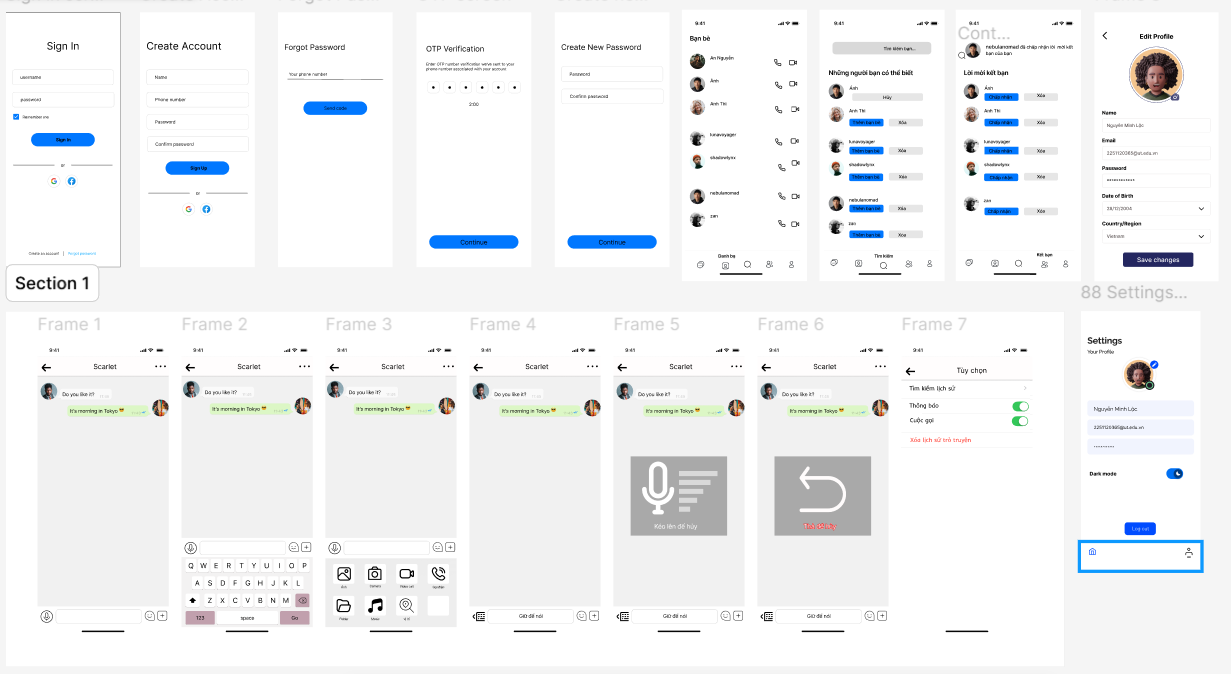
\includegraphics[width=0.7\textwidth]{giaodien.png}
		\end{center}
	\end{itemize}

	\vspace{0.5cm}
	\textbf{PHÂN TÍCH HỆ THỐNG} \\
	
	\textbf{4.1. Mô hình chức năng hệ thống} \\
	Mô hình chức năng mô tả các chức năng chính mà hệ thống nhắn tin cung cấp cho người dùng. Bao gồm:
	\begin{itemize}
		\item Đăng ký, đăng nhập tài khoản.
		\item Quản lý thông tin cá nhân.
		\item Gửi và nhận tin nhắn.
		\item Tạo nhóm trò chuyện và quản lý nhóm.
		\item Nhận thông báo khi có tin nhắn mới.
	\end{itemize}
	
	\textbf{4.2. Biểu đồ Use Case} \\
	Biểu đồ Use Case thể hiện các chức năng mà người dùng có thể tương tác với hệ thống:
	\begin{itemize}
		\item Người dùng có thể: đăng ký, đăng nhập, gửi/nhận tin nhắn, gọi điện, tạo nhóm, thêm/xóa thành viên nhóm.
		\item Hệ thống xử lý xác thực người dùng, lưu trữ và đồng bộ tin nhắn, gửi thông báo.
	\end{itemize}
	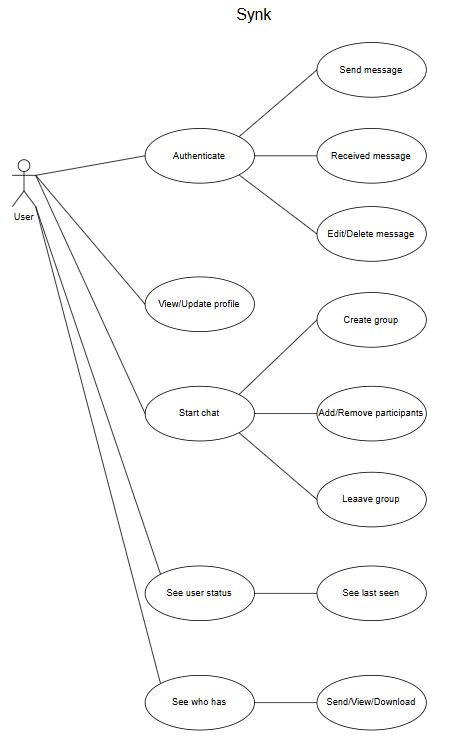
\includegraphics[width=0.7\textwidth]{usecase.png}\\[0.5cm]
	
	\textbf{4.3. Biểu đồ hoạt động} \\
	Biểu đồ hoạt động mô tả quy trình luồng hoạt động của một chức năng cụ thể, ví dụ gửi tin nhắn:
	\begin{enumerate}
		\item Người dùng nhập nội dung tin nhắn.
		\item Nhấn nút gửi.
		\item Hệ thống kiểm tra kết nối mạng.
		\item Nếu hợp lệ, tin nhắn được lưu vào cơ sở dữ liệu và gửi đến người nhận.
		\item Người nhận nhận được thông báo và xem nội dung.
	\end{enumerate}
	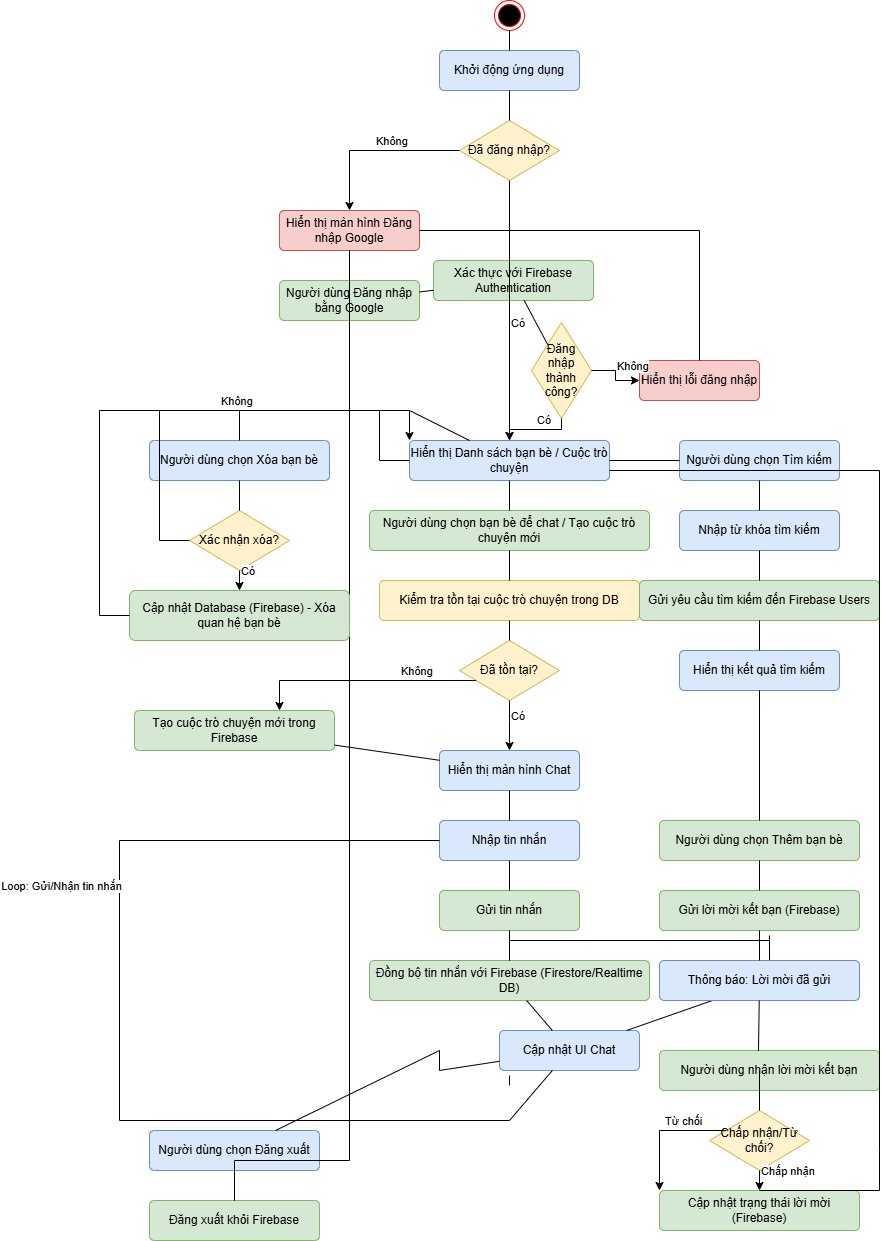
\includegraphics[width=0.7\textwidth]{sodo.png}\\[0.5cm]
	
	\textbf{4.4. Biểu đồ tuần tự} \\
	Biểu đồ tuần tự mô tả sự tương tác theo thời gian giữa các đối tượng trong hệ thống. Ví dụ trình tự khi gửi tin nhắn:
	\begin{enumerate}
		\item Người dùng nhấn gửi tin nhắn.
		\item Ứng dụng gửi yêu cầu tới server.
		\item Server xử lý, lưu trữ và trả kết quả.
		\item Tin nhắn được hiển thị trên giao diện người gửi và được đẩy tới người nhận.
	\end{enumerate}
	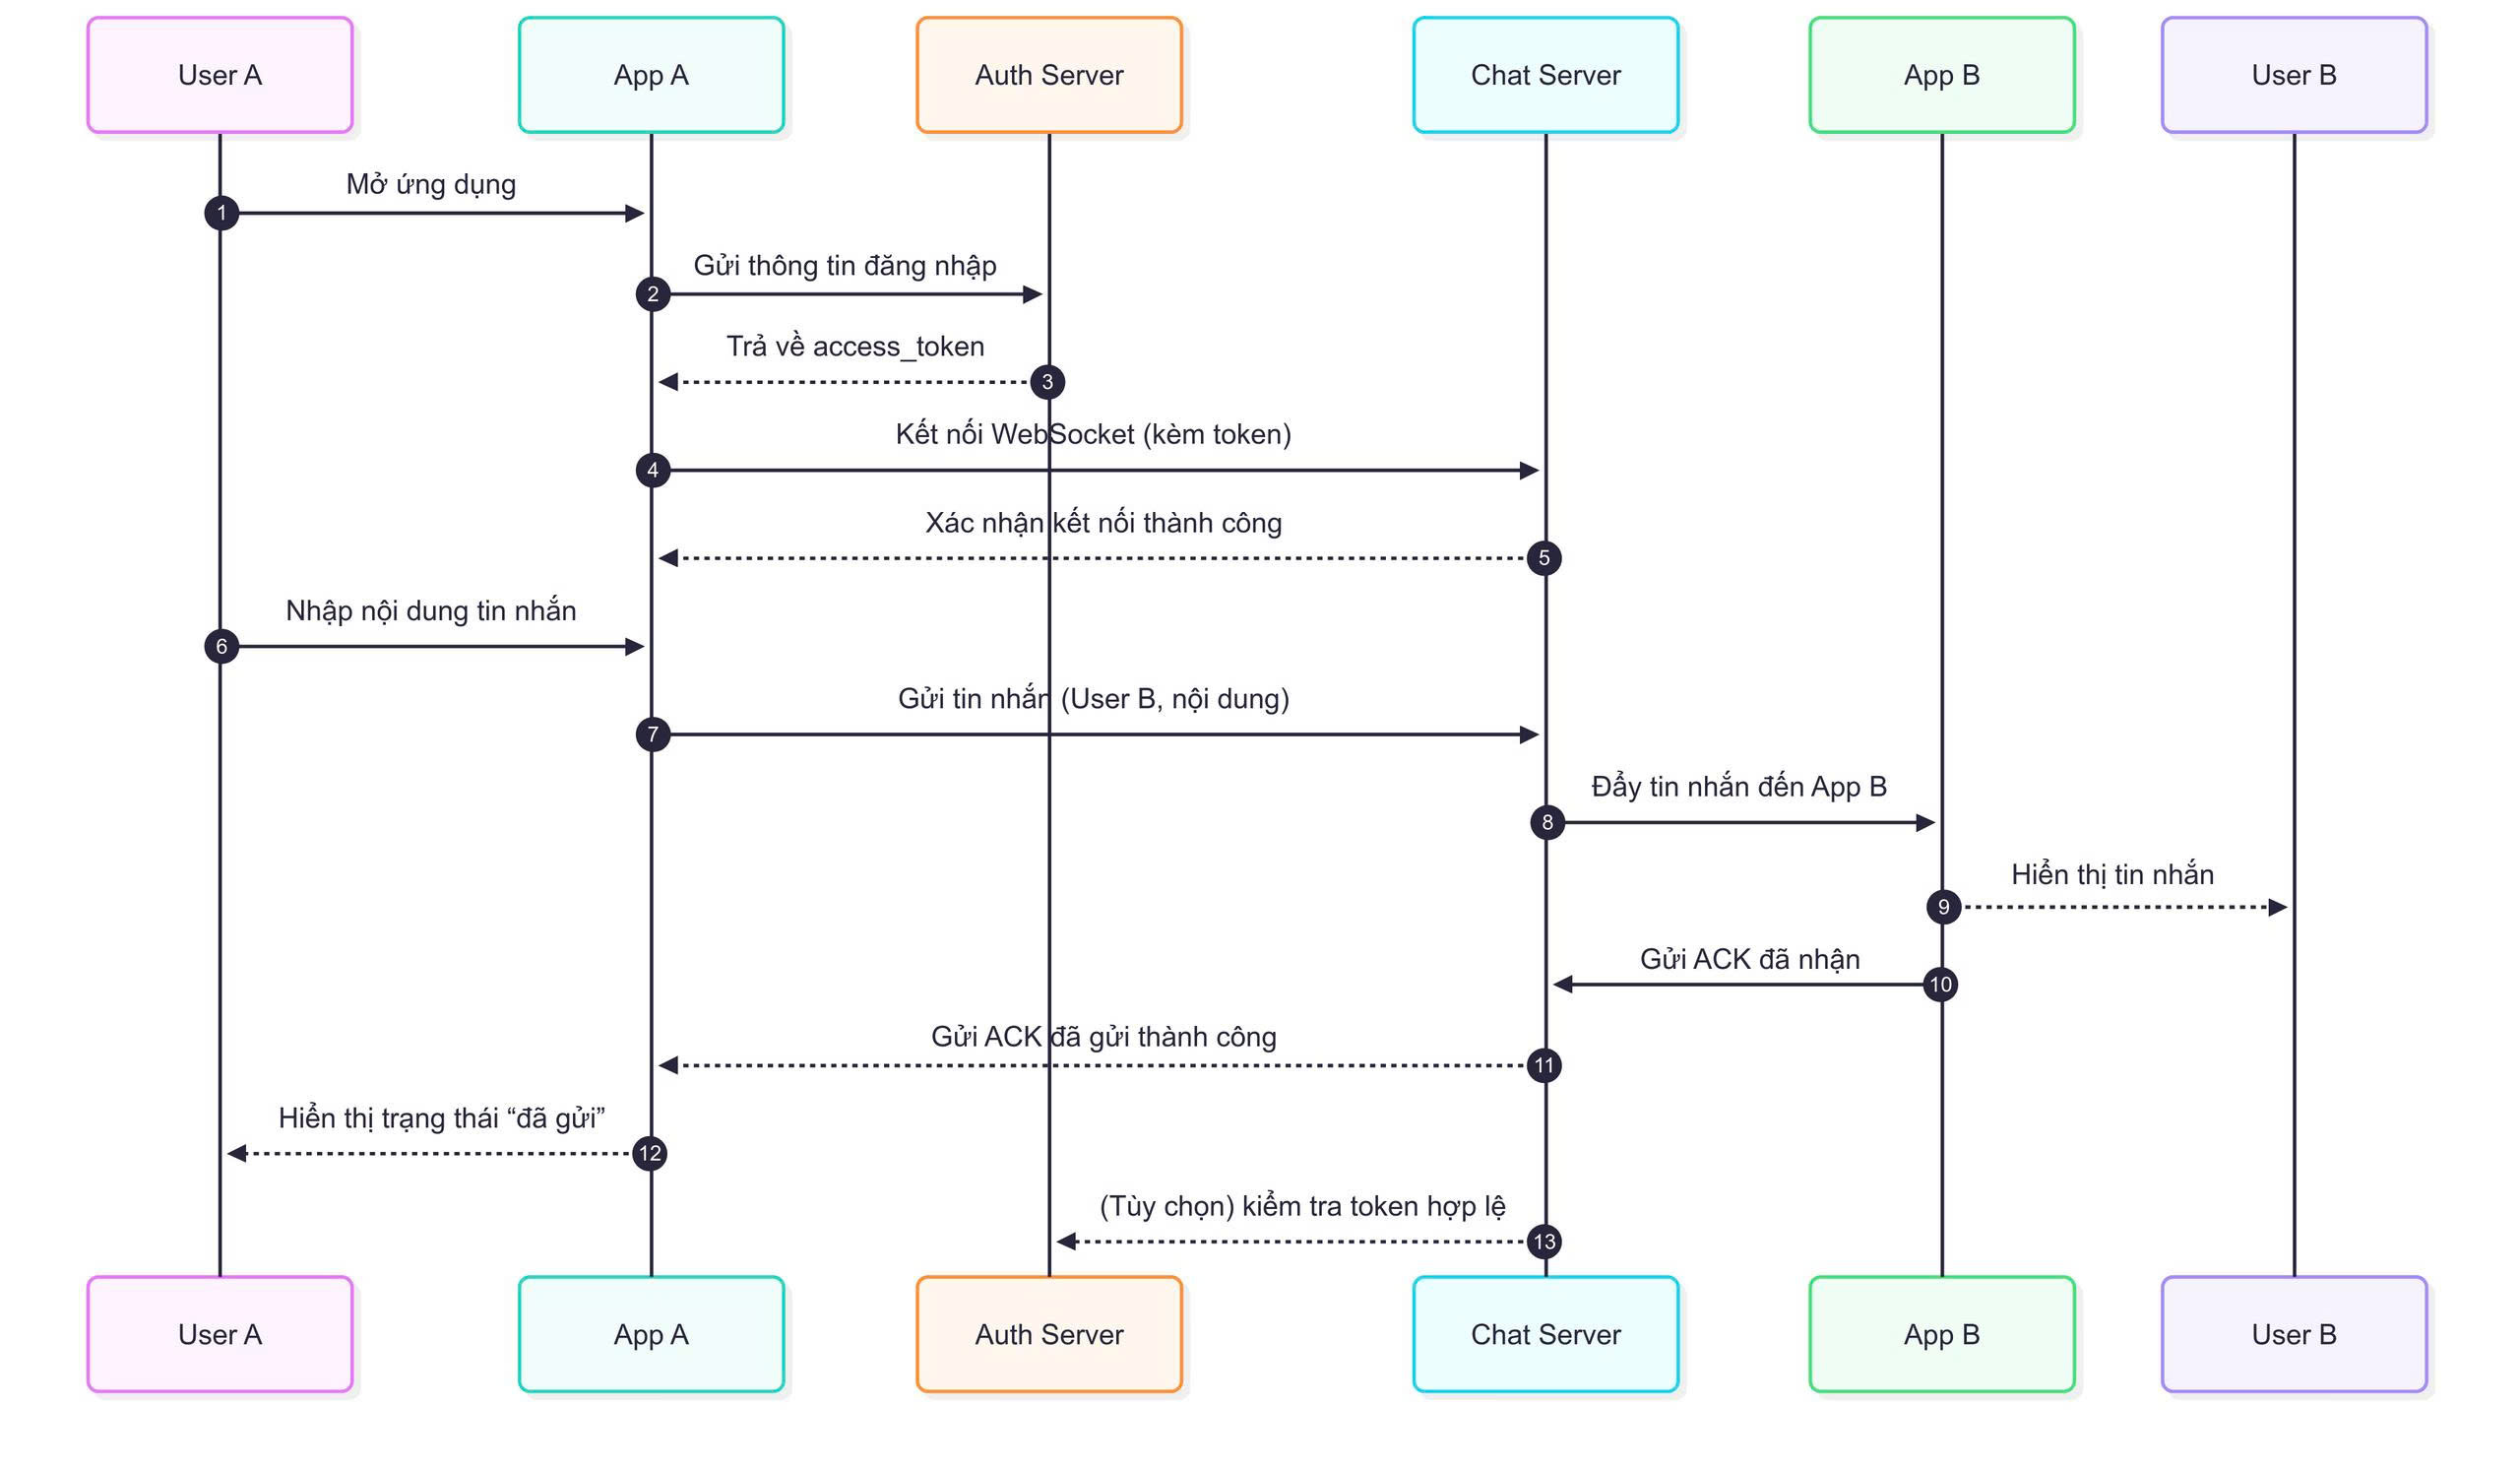
\includegraphics[width=0.7\textwidth]{sodotuantu.jpg}\\[0.5cm]
	
	\textbf{4.5. Mô hình dữ liệu người dùng, tin nhắn} \\
	Mô hình dữ liệu giúp xác định cách các thông tin được lưu trữ trong hệ thống.
	\begin{itemize}
		\item \textbf{Bảng người dùng (Users):} ID, tên đăng nhập, mật khẩu mã hóa, ảnh đại diện, trạng thái hoạt động.
		\item \textbf{Bảng tin nhắn (Messages):} ID tin nhắn, ID người gửi, ID người nhận/ID nhóm, nội dung, thời gian gửi, loại tin nhắn (văn bản, hình ảnh, âm thanh).
		\item \textbf{Bảng nhóm (Groups):} ID nhóm, tên nhóm, người tạo, thành viên.
	\end{itemize}
	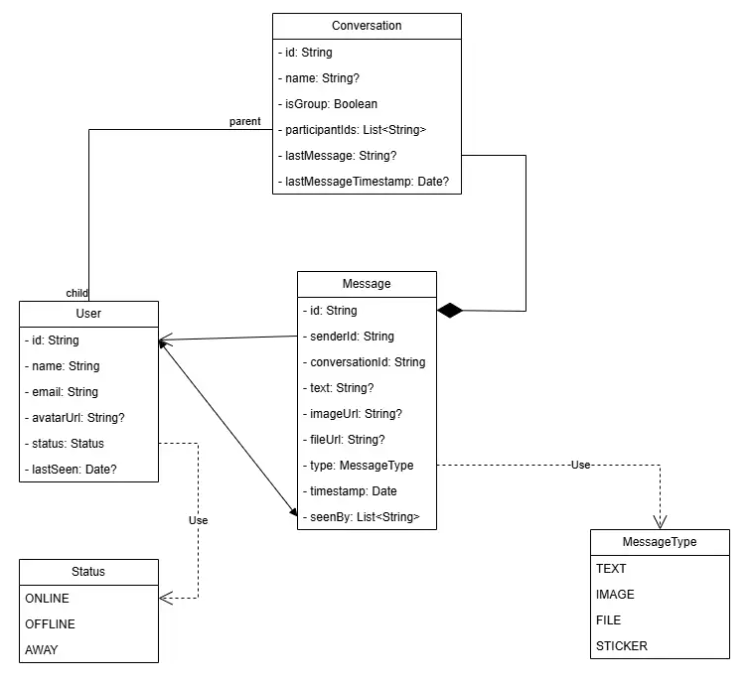
\includegraphics[width=0.7\textwidth]{hinhsodo.png}\\[0.5cm]
	\vspace{0.5cm}
	\clearpage
	\textbf{THIẾT KẾ HỆ THỐNG} \\
	
	\textbf{5.1. Kiến trúc hệ thống Client - Firebase} \\
	Hệ thống được thiết kế theo mô hình client-server, trong đó:
	\begin{itemize}
		\item \textbf{Client:} là ứng dụng Android viết bằng Kotlin, chịu trách nhiệm giao tiếp với người dùng, gửi và nhận dữ liệu.
		\item \textbf{Server:} sử dụng Firebase làm backend (Realtime Database hoặc Firestore, Firebase Auth, Storage), chịu trách nhiệm lưu trữ dữ liệu, xác thực, đồng bộ hóa theo thời gian thực.
	\end{itemize}
	Firebase giúp giảm thiểu thời gian phát triển nhờ vào các dịch vụ tích hợp sẵn như: Authentication, Realtime Database, Cloud Messaging, và Firebase Storage.
	
	\textbf{5.2. Thiết kế giao diện người dùng (UI/UX)} \\
	Ứng dụng được thiết kế thân thiện với người dùng, dễ sử dụng, ưu tiên trải nghiệm mượt mà. Các màn hình chính bao gồm:
	\begin{itemize}
		\item Màn hình đăng nhập/đăng ký.
		\item Màn hình danh sách bạn bè và nhóm chat.
		\item Màn hình trò chuyện cá nhân hoặc nhóm.
		\item Màn hình gửi hình ảnh/sticker.
		\item Màn hình cập nhật thông tin cá nhân.
	\end{itemize}
	Thiết kế sử dụng Material Design để tạo giao diện hiện đại, trực quan và đồng nhất.
	
	\textbf{5.3. Thiết kế cơ sở dữ liệu Firebase Realtime Database / Firestore} \\
	Dữ liệu được tổ chức theo cấu trúc dạng cây (với Realtime Database) hoặc dạng collection-document (với Firestore). Một số cấu trúc chính:
	\begin{itemize}
		\item \textbf{Users:} lưu thông tin người dùng như ID, tên, email, ảnh đại diện, trạng thái online/offline.
		\item \textbf{Messages:} lưu tin nhắn theo đoạn chat, gồm người gửi, nội dung, thời gian, loại tin nhắn (văn bản, ảnh…).
		\item \textbf{Groups:} lưu thông tin nhóm như tên nhóm, danh sách thành viên, lịch sử trò chuyện.
	\end{itemize}
	Cấu trúc được thiết kế để đảm bảo truy xuất nhanh, cập nhật theo thời gian thực và dễ mở rộng.
	
	\textbf{5.4. Luồng hoạt động của các chức năng:} \\
	
	\hspace*{1cm} \textbf{- Đăng ký/Đăng nhập} \\
	\hspace*{1cm} Người dùng nhập email và mật khẩu, hệ thống sử dụng Firebase Authentication để xác thực. Nếu hợp lệ, chuyển đến giao diện chính.
	
	\hspace*{1cm} \textbf{- Gửi/nhận tin nhắn} \\
	\hspace*{1cm} Tin nhắn được gửi lên Firebase, sau đó được đồng bộ đến thiết bị người nhận theo thời gian thực thông qua listener.
	
	\hspace*{1cm} \textbf{- Chat nhóm} \\
	\hspace*{1cm} Người dùng gửi tin vào nhóm, hệ thống lưu vào nhánh dữ liệu nhóm, tất cả thành viên nhóm đều nhận được tin nhắn mới.
	
	\hspace*{1cm} \textbf{- Gửi hình ảnh/sticker} \\
	\hspace*{1cm} Ảnh được tải lên Firebase Storage, sau đó hệ thống lưu đường dẫn ảnh vào phần nội dung tin nhắn để hiển thị.
	
	\hspace*{1cm} \textbf{- Trạng thái hoạt động của người dùng} \\
	\hspace*{1cm} Khi người dùng đăng nhập, ứng dụng cập nhật trạng thái “online” trong cơ sở dữ liệu. Khi thoát, trạng thái được cập nhật thành “offline” hoặc lưu thời gian hoạt động lần cuối.
	\vspace{0.5cm}
	
	\vspace{0.5cm}
	\noindent\textbf{CÀI ĐẶT HỆ THỐNG} \\
	
	\vspace{0.3cm}
	\noindent\textbf{6.1. Công cụ phát triển: Android Studio, Kotlin, Firebase} \\
	Ứng dụng được phát triển trên nền tảng Android Studio, sử dụng ngôn ngữ Kotlin cùng thư viện giao diện hiện đại Jetpack Compose. Jetpack Compose hỗ trợ xây dựng giao diện theo hướng khai báo, giúp mã nguồn ngắn gọn và dễ quản lý hơn so với XML truyền thống. Firebase được tích hợp để cung cấp các dịch vụ xác thực người dùng, lưu trữ dữ liệu và chia sẻ đa phương tiện, bao gồm:
	\begin{itemize}
		\item Hệ thống xác thực người dùng.
		\item Cơ sở dữ liệu thời gian thực cho tin nhắn.
		\item Lưu trữ và chia sẻ hình ảnh hoặc sticker.
	\end{itemize}
	
	\vspace{0.3cm}
	\noindent\textbf{6.2. Cài đặt giao diện người dùng bằng Jetpack Compose} \\
	Giao diện ứng dụng được xây dựng hoàn toàn bằng Jetpack Compose mà không sử dụng file XML. Mỗi màn hình được thiết kế theo mô hình khai báo, với trạng thái được quản lý chặt chẽ. Các thành phần giao diện chính bao gồm màn hình đăng nhập, đăng ký, danh sách trò chuyện và khu vực nhắn tin, được tổ chức rõ ràng và hỗ trợ điều hướng linh hoạt.
	
	\vspace{0.3cm}
	\noindent\textbf{6.3. Cài đặt kết nối Firebase Authentication} \\
	Hệ thống đăng ký và đăng nhập người dùng được tích hợp bằng dịch vụ xác thực của Firebase. Quá trình đăng ký và đăng nhập được xử lý tách riêng phần giao diện và logic, đảm bảo người dùng có trải nghiệm mượt mà. Trạng thái đăng nhập được theo dõi và cập nhật tự động lên giao diện.
	
	\vspace{0.3cm}
	\noindent\textbf{6.4. Cài đặt lưu trữ và đồng bộ tin nhắn bằng Firestore} \\
	Tin nhắn của người dùng được lưu trữ trong Firestore với khả năng đồng bộ thời gian thực. Khi người dùng gửi hoặc nhận tin nhắn, dữ liệu được tự động cập nhật và hiển thị ngay trên giao diện mà không cần tải lại. Cấu trúc dữ liệu được thiết kế để dễ dàng mở rộng và quản lý.
	
	\vspace{0.3cm}
	\noindent\textbf{6.5. Gửi và nhận hình ảnh qua Firebase Storage} \\
	Ứng dụng cho phép người dùng gửi và nhận hình ảnh thông qua Firebase Storage. Khi một hình ảnh được tải lên, hệ thống lưu trữ trên nền tảng đám mây và chia sẻ liên kết trong tin nhắn. Ảnh được hiển thị ngay trong giao diện trò chuyện, đảm bảo trải nghiệm nhắn tin trực quan và sinh động.
	
	\textbf{KIỂM THỬ ỨNG DỤNG} \\
	
	\textbf{7.1. Mục tiêu kiểm thử} \\
	Mục tiêu của quá trình kiểm thử là đảm bảo ứng dụng hoạt động ổn định, đúng chức năng, giao diện thân thiện và phản hồi nhanh. Kiểm thử cũng giúp phát hiện lỗi trong quá trình xử lý dữ liệu, đăng nhập, nhắn tin và các chức năng phụ trợ.
	
	\textbf{7.2. Kiểm thử chức năng} \\
	Các chức năng chính được kiểm thử bao gồm:
	\begin{itemize}
		\item \textbf{Đăng ký/Đăng nhập}: Kiểm tra việc xác thực người dùng với Firebase Authentication.
		\item \textbf{Gửi/nhận tin nhắn}: Đảm bảo tin nhắn hiển thị theo thời gian thực, đúng thứ tự.
		\item \textbf{Chat nhóm}: Nhiều người dùng có thể gửi và nhận tin nhắn cùng lúc.
		\item \textbf{Gửi hình ảnh}: Hình ảnh được chọn từ thiết bị và tải lên Firebase Storage thành công.
		\item \textbf{Trạng thái người dùng}: Kiểm tra tính năng "online/offline" hoạt động chính xác.
	\end{itemize}
	
	\textbf{7.3. Kiểm thử giao diện} \\
	Vì ứng dụng sử dụng Jetpack Compose nên việc kiểm thử giao diện tập trung vào:
	\begin{itemize}
		\item Đảm bảo UI phản ứng tốt với các trạng thái khác nhau của dữ liệu (`State` và `LiveData`).
		\item Kiểm tra khả năng tương thích với nhiều kích thước màn hình.
		\item Kiểm tra hiệu suất cuộn của `LazyColumn` trong danh sách tin nhắn.
		\item Kiểm tra khả năng điều hướng giữa các màn hình qua `Navigation Compose`.
	\end{itemize}
	
	\textbf{7.4. Kết quả kiểm thử và đánh giá} \\
	Quá trình kiểm thử được thực hiện trên nhiều thiết bị Android với phiên bản khác nhau. Kết quả cho thấy:
	\begin{itemize}
		\item Các chức năng hoạt động ổn định, tốc độ phản hồi nhanh.
		\item Giao diện người dùng dễ sử dụng, phù hợp với người dùng phổ thông.
		\item Một số lỗi nhỏ như: tải ảnh chậm khi mạng yếu, trạng thái người dùng chưa cập nhật ngay tức thì.
	\end{itemize}
	Tổng thể, ứng dụng đáp ứng yêu cầu ban đầu và đạt mức độ hoàn thiện cao ở phiên bản đầu tiên.
	
	\vspace{0.5cm}
	\textbf{KẾT LUẬN VÀ HƯỚNG PHÁT TRIỂN} \\
	
	\textbf{8.1. Kết quả đạt được} \\
	Đề tài đã xây dựng thành công một ứng dụng nhắn tin đơn giản với các tính năng cơ bản: đăng ký, đăng nhập, gửi/nhận tin nhắn, gửi hình ảnh, quản lý người dùng và trạng thái hoạt động. Giao diện được xây dựng bằng Jetpack Compose hiện đại, mang lại trải nghiệm mượt mà. Firebase được sử dụng làm nền tảng lưu trữ dữ liệu hiệu quả.
	
	\textbf{8.2. Hạn chế của phần mềm} \\
	\begin{itemize}
		\item Chưa có mã hóa dữ liệu đầu cuối (end-to-end encryption).
		\item Ứng dụng chưa có thông báo đẩy khi có tin nhắn mới.
		\item Tốc độ tải ảnh có thể chậm trong môi trường mạng yếu.
		\item Chưa hỗ trợ gọi video/âm thanh.
	\end{itemize}
	
	\textbf{8.3. Hướng phát triển trong tương lai} \\
	Trong tương lai, ứng dụng có thể được mở rộng với các tính năng nâng cao:
	\begin{itemize}
		\item \textbf{Thông báo đẩy (Push Notification)}: Sử dụng Firebase Cloud Messaging để thông báo khi có tin nhắn mới.
		\item \textbf{Mã hóa tin nhắn}: Áp dụng kỹ thuật mã hóa đầu cuối (E2EE) để đảm bảo quyền riêng tư người dùng.
		\item \textbf{Tối ưu lưu trữ}: Giảm kích thước ảnh trước khi tải lên Storage.
		\item \textbf{Giao diện nâng cao}: Thêm chế độ tối (dark mode), biểu tượng cảm xúc tùy chỉnh.
		\item \textbf{Tính năng gọi video/âm thanh}: Tích hợp WebRTC hoặc các SDK bên thứ ba như Agora.
	\end{itemize}
	\noindent\textbf{\Large TÀI LIỆU THAM KHẢO}
	
	\vspace{0.5cm}
	
	\begin{enumerate}
		\item kotlin-scratch-project-programmer
		\item Head First Android Development, 3rd Edition
		\item ChatGPT (OpenAI)
	\end{enumerate}
	
	
	
	
	
\end{document}
